\pdfoutput=1
%cmt: NSF IIS-1250985 and NSF IIS-1407939
\documentclass[11pt,letterpaper]{article}
\usepackage{naaclhlt2015}
\usepackage{times}
\usepackage{latexsym}
%\usepackage{hhline}

\usepackage{epstopdf}
%\usepackage{fullpage,times,color}
\usepackage[ruled]{algorithm2e}
\usepackage{graphicx}
%\usepackage{hyperref}
\usepackage{multirow}
\usepackage{url}
\usepackage{subcaption}
\usepackage{amsmath,amsthm,amssymb}

%\graphicspath{{figures/}} 

\newtheorem{assumption}{Assumption}
\newtheorem{definition}{Definition}
\newtheorem{theorem}{Theorem}

\newcommand{\cmt}[1]{{\em #1}}

\newcommand{\cX}{{\mathcal X}}
\newcommand{\cY}{{\mathcal Y}}

\newcommand{\cnn}{CNN}

\newcommand{\scnnpfx}{seq}
\newcommand{\bcnnpfx}{bow}
\newcommand{\scnn}{seq-CNN}
\newcommand{\sscnn}{seq2-CNN}
\newcommand{\ssbcnn}{seq2-bow$n$-CNN}

\newcommand{\sconv}{seq-convolution}
\newcommand{\sconvAdj}{seq-convolutional}
\newcommand{\bcnn}{bow-CNN}
\newcommand{\bconv}{bow-convolution}
\newcommand{\bconvAdj}{bow-convolutional}

\newcommand{\bowf}{f_{\rm bow}}
\newcommand{\bow}{{bow}}
\newcommand{\bowone}{{bow1}}
\newcommand{\bowtwo}{{bow2}}
\newcommand{\bowthree}{{bow3}}
\newcommand{\bongram}{bag-of-$n$-gram}
\newcommand{\bongrams}{bag-of-$n$-grams}

\newcommand{\bx}{{\mathbf x}}
\newcommand{\bz}{{\mathbf z}}
\newcommand{\bw}{{\mathbf w}}

\newcommand{\psz}{p}
\newcommand{\doc}{D}
\newcommand{\voc}{V}
\newcommand{\vsz}{|\voc|}
\newcommand{\wrd}{w}
\newcommand{\dsz}{|\doc|}

\newcommand{\Activ}{\boldsymbol{\sigma}}
\newcommand{\activ}{\sigma}
\newcommand{\ip}[2]{{#1} \cdot {#2}} % inner product
\newcommand{\Ip}[2]{{#1} \cdot {#2}} 
\newcommand{\bias}{b}
\newcommand{\wei}{\bw}
\newcommand{\Wei}{{\mathbf W}}
\newcommand{\Bias}{{\mathbf b}}
\newcommand{\region}{{\mathbf r}} % a small region 
\newcommand{\iL}{\ell} % location index
\newcommand{\nL}{L}
\newcommand{\iB}{i}     % bank index (or weight index)
\newcommand{\ind}{{\cal I}}

\newcommand{\Elec}{Elec} 

\setlength{\textfloatsep}{2ex}
\setlength{\floatsep}{2ex}
%\setlength{\abovecaptionskip}{1ex}
%\setlength{\belowcaptionskip}{1ex}

\newcommand{\bEqsz}{\begin{small}}
\newcommand{\eEqsz}{\end{small}}
%\newcommand{\bEqsz}{\begin{footnotesize}}
%\newcommand{\eEqsz}{\end{footnotesize}}

\newcommand{\nbw}{NB-LM}

\makeatletter
\newcommand\tightpara{\@startsection{paragraph}{4}{\z@}{1ex plus
   0ex minus 0.2ex}{-1em}{\normalsize\bf}}
%---  as in naaclhlt2015.sty
\newcommand\normalpara{\@startsection{paragraph}{4}{\z@}{1.5ex plus
   0.5ex minus .2ex}{-1em}{\normalsize\bf}}
\makeatother   
   
   
\title{Effective Use of Word Order for Text Categorization \\ with Convolutional Neural Networks\thanks{
To appear in NAACL HLT 2015. 
}}
\renewcommand\footnotemark{}
%\renewcommand\footnoterule{}
\author{Rie Johnson\\
	    RJ Research Consulting\\
	    Tarrytown, NY, USA\\
	    {\tt riejohnson@gmail.com}
	  \And
	Tong Zhang\\
    Baidu Inc., Beijing, China \\    
    Rutgers University, Piscataway, NJ, USA \\
  {\tt tzhang@stat.rutgers.edu}
}
\date{}
\begin{document}
\maketitle
\begin{abstract}
Convolutional neural network (\cnn) is a neural network that can make use of 
the internal structure of data such as the 2D structure of image data.  
This paper studies \cnn\ on text categorization to exploit
the 1D structure (namely, word order) of text data for accurate prediction.  
Instead of using low-dimensional word vectors as input as is often done, 
we directly apply \cnn\ to high-dimensional text data, which leads to 
directly learning embedding of small text regions for use in classification.  
In addition to a straightforward adaptation of \cnn\ from image to text, 
a simple but new variation which employs bag-of-word conversion in the 
convolution layer is proposed.  
%Two types of \cnn\ are studied: 
%a straightforward adaptation of \cnn\ from image to text, % (\scnn), 
%and a simple but new variation % \bcnn\
%which employs bag-of-word conversion in the 
%convolution layer.  
An extension to combine multiple convolution layers is also explored for higher 
accuracy.    
The experiments demonstrate the effectiveness of our approach in comparison with 
state-of-the-art methods.
%, as well as with 
%previous \cnn\ models for text 
%which are more complex and expensive to train. % than ours. 

%In our experiments, \bcnn\ outperforms \scnn\ on topic classification, 
%vice versa on sentiment classification, and both outperform 
%the traditional \bongram\ vector-based methods and previous \cnn\ models for text, 
%which are more complex and expensive to train. % than ours.  
%We empirically show that 
%\cnn\ can make more effective use of high-order $n$-grams than the standard methods 
%with \bongram\ vectors. 
%Better results than the previous supervised results on % the benchmarking datasets 
%RCV1 and IMDB are reported. 
\end{abstract}

%*********************
\section{Introduction}

Text categorization is the task of automatically assigning pre-defined categories to 
documents written in natural languages.  
Several types of text categorization have been studied, each of which deals with 
different types of documents and categories, 
such as topic categorization to detect discussed topics (e.g., sports, politics), 
spam detection \cite{SDHH98}, % to filter out spam emails, 
and sentiment classification \cite{PLV02,PL08,MDPHNP11} 
to determine %whether the sentiment is positive or 
%negative, typically applied to product reviews or movie reviews.  
the sentiment typically in product or movie reviews.  
%
A standard approach to text categorization 
is to represent documents by {\em bag-of-word vectors}, 
namely, vectors that indicate which words appear in the documents but do not preserve
word order, and use classification models such as % Support Vector Machines % \cite{Vapnik95}
SVM. %  or Max Entropy. 
%, naive Bayes, decision trees, and Max Entropy. 

It has been noted that loss of word order caused by bag-of-word vectors 
({\em \bow\ vectors}) is particularly problematic on sentiment classification.  
%\footnote{
%  For example, it may be hard to distinguish the positive sentiment in 
%  ``It's a good movie.'' from the negative sentiment in ``It's not a good movie at all.''
%  once the words of these sentences are thrown into `bags' with the rest of the respective   
%  documents.  
%}.  
A simple remedy is to use word bi-grams in addition to uni-grams 
\cite{BDP07,GBB11,WM12}. 
However, 
use of word $n$-grams with $n>1$ on text categorization in general is not always 
effective; e.g.,   
%\newcite{WM12} report that use of tri-grams on sentiment classification 
%slightly hurt performance; 
on topic categorization, simply adding phrases or $n$-grams 
is not effective (see, e.g., references in \cite{TWL02}).  

To benefit from word order on text categorization, 
we take a different approach, 
%Instead of using bags of $n$-grams, 
which employs {\em convolutional neural networks (\cnn)}
\cite{LeCun+etal98}. 
%,C+etal11}.  
%---
\cnn\ is a neural network that can make use of the internal structure of data 
such as the {\em 2D structure} of image data through convolution layers, 
where each computation unit responds to a small region of input data 
(e.g., a small square of a large image).  We apply \cnn\ to text 
categorization to make use of the {\em 1D structure} (word order) 
of document data so that each unit in the convolution layer responds to 
a small region of a document (a sequence of words).

\cnn\ has been very successful on image classification; see e.g., 
the winning solutions of ImageNet Large Scale Visual Recognition Challenge 
 \cite{imagenetNips12,Szegedy+etal14,Russakovsky+etal14}.  % ZF13
%---  not true any more ... 
%there have been only a few applications of \cnn\ to text data, and these have been 
%token-level applications (i.e., output is per token) \cite{nnnlpICML08,nnnlpJMLR11}. 

%---
%In the NLP field, 
On text, 
since the work on token-level applications (e.g., POS tagging) by 
%\cite{nnnlpICML08,nnnlpJMLR11}, 
\newcite{nnnlpJMLR11}, 
\cnn\ has been used in systems for 
entity search,  %\cite{Gao+etal14}, % automatic highlighting, 
sentence modeling, %\cite{KGB14,Kim14}, 
word embedding learning, %\cite{WCA14,Tang+etal14}, 
product feature mining, % \cite{XLLZ14} 
%information retrieval \cite{Shen+etal14},
and so on 
\cite{XS13,Gao+etal14,Shen+etal14,KGB14,XLLZ14,Tang+etal14,WCA14,Kim14}.  
%However, 
%in these recent studies, often \cnn\ is part of a larger 
%complex system, or \cnn\ is aided in a semi-supervised fashion 
%through word embeddings learned by some other method, 
%and the benefit of \cnn\ itself is often not clear.  
%-----
Notably, in many of these \cnn\ studies on text, 
%including studies in sentence classification  
%(which is related to document categorization), 
the first layer of the network converts words in sentences 
to {\em word vectors} by table lookup.  
The word vectors are either trained as part of \cnn\ training, or 
fixed to those learned by some other method 
(e.g., word2vec \cite{wvecNips13}) from an additional large corpus.  
The latter is a form of semi-supervised learning, which we study elsewhere. 
We are interested in the effectiveness of \cnn\ itself 
{\em without aid of additional resources}; therefore, 
word vectors should be trained as part of network training 
if word vector lookup is to be done.  
%
%Though it is usually called a word vector lookup layer, it is in fact 
%equivalent to a convolution layer with region size 1, stride 1, 
%$d$ computation units for producing $d$-dim word vectors, and no pooling. 

A question arises, however, whether word vector lookup in a purely supervised setting 
is really useful for text categorization.  
%If one implements \cnn\ without efficient handling of sparse data, 
%it is indeed necessary, for computational feasibility, to lower the dimensionality, 
%e.g., from 30K-dim one-hot vector to 100-dim word vector.  
%%by word vector lookup.  
%Other than that, word vector conversion in this setting seems rather unjustified.  
The essence of convolution layers is to {\em convert text regions 
of a fixed size (e.g., ``am so happy'' with size 3) to feature vectors}, as described later. 
In that sense, a word vector learning layer is a special (and unusual) case of convolution layer with 
region size one.  
Why is size one appropriate if bi-grams are more discriminating than uni-grams? 
%Given the fact that word sequences are more discriminating than individual words, 
%why should we use individual words in the first stage, 
%deferring use of word sequences to the next layer?  
%
Hence, we take a different approach.  
We {\em directly apply \cnn\ to high-dimensional one-hot vectors};  
i.e., we {\em directly} learn {\em embedding}\footnote{
  We use the term `embedding' loosely to mean a structure-preserving function, 
  in particular, a function that generates low-dimensional features 
  that preserve the predictive structure. 
} of text regions without going through word embedding learning.  
This approach is made possible by solving the computational issue\footnote{
  \cnn\ implemented for image would not handle sparse data efficiently, and 
  without efficient handling of sparse data, 
  convolution over high-dimensional one-hot vectors would be computationally infeasible. 
}
through efficient handling of high-dimensional sparse data 
% (i.e., memory is allocated for and arithmetic is done over the nonzero components only) 
on GPU, and 
%\footnote{ 
%  A side product of this work is the high-speed \cnn\ code on GPU 
%  that efficiently handles sparse high-dimensional text data, made available 
%  for further research. 
%}, and 
%compared with word-vector-based \cnn, 
it turned out to have the merits of 
improving accuracy 
with fast training/prediction 
and simplifying the system (fewer hyper-parameters to tune).  
%cmt: saving space ...
%Training/prediction can be faster with efficient handling of sparse data 
%since high-dimensional one-hot vectors have a much fewer number of non-zero components than 
%low-dimensional dense word vectors.  
Our 
%This high-speed  %cmt: maybe too much boasting
\cnn\ code for text is publicly available on the internet\footnote{
  \url{riejohnson.com/cnn_download.html}
}.  

%The goal of this paper is to   % too long 
We 
study the effectiveness of \cnn\
%with minimum adaptation from the original \cnn\ for image, 
on text categorization and explain why \cnn\ is suitable for the task.  
Two types of \cnn\ are tested: 
{\em \scnn} is a straightforward adaptation of \cnn\ from image to text, and 
{\em \bcnn} is a simple but new variation of \cnn\ that employs bag-of-word conversion 
in the convolution layer.  
%to counteract a potential shortcoming of \scnn.  
The experiments show that \scnn\ outperforms \bcnn\ on sentiment classification, 
vice versa on topic classification, 
and the winner generally outperforms the conventional \bongram\ vector-based methods, as well as 
previous \cnn\ models for text which are more complex. 
%cmt: speed depends on implementation details.  previous models (kgn14,kim14) are so expensive to train 
%  partly because they are treating sentences as fixed-length text by zero padding.  
%                   
In particular, to our knowledge, this is the first work that has successfully used 
word order to % significantly  
improve topic classification performance.  
%In particular, we report 
%better results than the previous supervised results on two benchmarking datasets: 
%RCV1 for topic categorization and IMDB for sentiment classification.  
%
A simple extension that combines multiple convolution layers (thus 
combining multiple types of text region embedding) 
leads to further improvement.  
Through empirical analysis, we will show that 
\cnn\ can make effective use of high-order $n$-grams when conventional methods fail.  
%because 
%with \cnn, $n$-grams 
%can contribute to accurate prediction {\em even if they did not appear in the training data}.  

%*******************************
%\section{Convolutional neural networks for document classification}
\section{\cnn\ for document classification}
\label{sec:method}
 
We first review \cnn\ applied to image data and then 
discuss the application of \cnn\ to document classification tasks 
to introduce \scnn\ and \bcnn.  

%+++++++++++++++++++++++++++++++++++++++
\begin{figure}
\centering
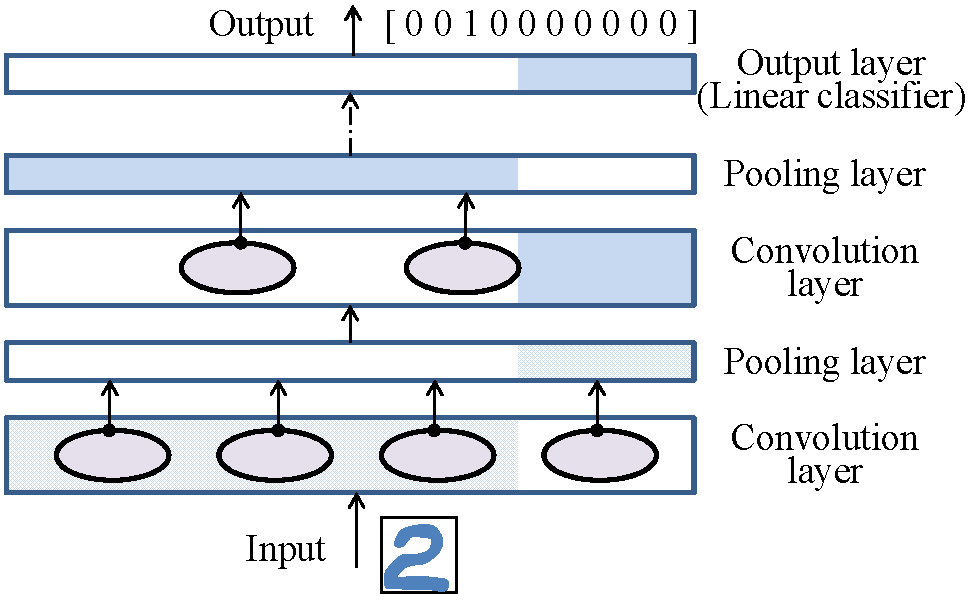
\includegraphics[width=2.6in]{cnn}
\vspace{-0.1in}
\caption{\label{fig:cnn} \small
Convolutional neural network.  % Ovals are computation units.  
}
\end{figure}
%+++++++++++++++++++++++++++++++++++++++

%----
\subsection{Preliminary: \cnn\ for image}
\label{sec:cnn-image}

%+++++++++++++++++++++++++++++++++++++++
\begin{figure}
\centering
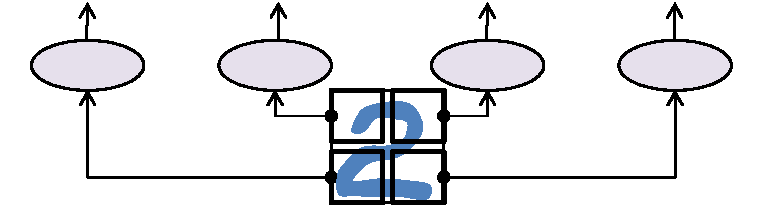
\includegraphics[width=2in]{imgconv}
\vspace{-0.1in}
\caption{\label{fig:imgconv} \footnotesize % \small
Convolution layer for image.  
Each computation unit (oval) computes a non-linear function 
$\Activ( \Wei \cdot \region_\iL(\bx) + \Bias )$ of a small region $\region_\iL(\bx)$ of input image $\bx$, 
where weight matrix $\Wei$ and bias vector $\Bias$ are shared by all the units in the same layer.
}
\end{figure}
%+++++++++++++++++++++++++++++++++++++++

\cnn\ is a feed-forward neural network with convolution layers interleaved with  
pooling layers, as illustrated in Figure \ref{fig:cnn}, where 
the top layer performs classification using the features generated by the 
layers below. % through non-linear operations.  
%%
%\paragraph{Sparse connectivity}
A convolution layer consists of several computation units, each of which 
takes as input a {\em region vector} that represents a small region of the input image 
and applies a non-linear function to it.  
Typically, the region vector is a concatenation of pixels in the region, which 
would be, for example, 75-dimensional if the region is $5 \times 5$ and the number of {\em channels} 
is three (red, green, and blue).  
Conceptually, computation units are placed over the input image so that the entire image is 
collectively covered, as illustrated in Figure \ref{fig:imgconv}.  
The region stride (distance between the region centers) is often set to a small value such as 1 
so that regions overlap with each other, 
though the stride in Figure \ref{fig:imgconv} is set larger than the region size for illustration.  
%To cover the pixels near the edges as adequately as the pixels in the center, 
%{\em padding} (with 0-value pixels) is often added to surround the image.  

%\paragraph{Shared weights} 
A distinguishing feature of convolution layers is {\em weight sharing}. 
%by the units 
%(or {\em tied weights}).  
%For example, suppose that $\Wei$ is a matrix whose rows are weight vectors 
%and $\Bias$ is a vector whose components are biases.  
%Then, 
Given input $\bx$, a unit associated with the $\iL$-th region computes 
%\begin{align*}
$
\Activ(\ip{\Wei}{\region_\iL(\bx)}+\Bias), 
$
%\label{eqn:convolution}
%\end{align*}
where $\region_\iL(\bx)$ is a region vector representing the region of $\bx$ 
at location $\ell$, 
and $\Activ$ is a pre-defined component-wise non-linear activation function, 
(e.g., applying $\activ(x)=\max(x,0)$ to each vector component).  
The matrix of {\em weights} $\Wei$ and the vector of {\em biases} $\Bias$ are 
learned through training, and they are {\em shared} by the computation units 
in the same layer.  
%\footnote{
%  Another way to describe a convolution layer is that there are {\em banks} of neurons 
%  so that in each bank neurons collectively cover the image and share a {\em weight vector} 
%  and a {\em bias}, and that banks share the placement of neurons.  
%  That is, a computation unit in our terminology corresponds to a group of neurons.  
%}. 
This weight sharing enables learning 
useful features irrespective of their location, while preserving the 
location where the useful features appeared.  

\newcommand{\numNeurono}{m}
\newcommand{\numNeuron}{$\numNeurono$}
%\paragraph{Pooling}
We regard the output of a convolution layer as an `image' so that the output of 
each computation unit is considered to be a `pixel' of \numNeuron\ channels 
where \numNeuron\ is the number of weight vectors (i.e., the number of 
rows of $\Wei$) or the number of {\em neurons}. 
In other words, {\em a convolution layer converts image regions to 
\numNeuron-dim vectors}, % where \numNeuron\ is the number of neurons, 
and the locations of the regions are inherited through this conversion.  
%and the \numNeuron-dim vectors inherit the locations of the original regions.  
%}.  
%

The output image of the convolution layer is passed to a pooling layer, 
which essentially shrinks the image by merging neighboring pixels, so that higher layers can deal with 
more abstract/global information.  
A pooling layer consists of pooling units, each of which is associated with a small region 
of the image.  %, and they collectively cover the entire image.  
Commonly-used merging methods are average-pooling and max-pooling, 
which respectively compute the channel-wise average/maximum of each region.  
%In other words, a pooling layer shrinks an image by merging neighboring pixels.  

%The output image is passed to the next layer, which may be another convolution layer; 
%in the end, the output layer computes the output from the final image by taking the 
%inner products with weight vectors.  

%To apply \cnn\ to image data, it is customary to fix the size and shape of image and the number of 
%channels (e.g., $256 \times 256$ pixels with three channels for RGB) 
%in advance so that the number of computation units in the convolution layer is fixed.  
%A pooling layer is typically designed so that it has a fixed number of pooling units 
%each of which is associated with a region of fixed size placed with a fixed stride.  
%This is possible because the size and the shape of all the input images is fixed in advance.  

%---------------------------
\subsection{\cnn\ for text} 
\label{sec:cnn-text}

Now we consider application of \cnn\ to text data.  
Suppose that we are given a document $\doc=(\wrd_1, \wrd_2, \ldots)$ with vocabulary 
$\voc$.  
\cnn\ requires vector representation of data that preserves internal locations (word order in this case) 
as input.  
A straightforward representation 
would be to treat each word as a pixel, treat 
$\doc$ as if it were an image of $\dsz \times 1$ pixels with $\vsz$ channels, 
and to represent each pixel (i.e., each word) as a $\vsz$-dimensional one-hot vector\footnote{
  Alternatively, one could use {\em bag-of-letter-n-gram vectors} as in \cite{Shen+etal14,Gao+etal14} 
  to cope with out-of-vocabulary words and typos.  
}. 
% , and that is what we do in this work.  
As a running toy example, 
suppose that vocabulary $\voc=\{$ ``don't'', ``hate'', ``I'', ``it'', ``love'' $\}$ 
and we associate the words with dimensions of vector in alphabetical order (as shown), 
and that document $\doc$=``I love it''.  
Then, we have a document vector: 
%\begin{small}
%\bEqsz
\vspace{-0.1in}
\[
  \bx=\left[~0~0~1~0~0~|~0~0~0~0~1~|~0~0~0~1~0~\right]^\top~. 
\]
%\end{small}
%\eEqsz

%----
\subsubsection{\scnn\ for text}
\label{sec:scnn}

As in the convolution layer for image, we 
represent each region (which each computation unit responds to) 
by a concatenation of the pixels, 
which makes $\psz\vsz$-dimensional region vectors where $\psz$ is the region size 
fixed in advance.  
For example, on the example document vector $\bx$ above, with $\psz=2$ and stride 1, 
we would have two regions 
``I love'' and ``love it'' represented by the following vectors: 
%\vspace{-0.1in}
%\vspace{-0.075in}
\[
\bEqsz
\region_0(\bx)=  %\bx[0:9]=
\left[ 
  \begin{array}{c} 0 \cr 0 \cr{\bf 1}\cr 0 \cr 0 \cr \mbox{---} \cr 0 \cr 0 \cr 0 \cr 0 \cr {\bf 1} \cr \end{array} 
\right]
\hspace{-0.1in}
  \begin{array}{c} {\rm don't}\cr{\rm hate}\cr{\rm \bf I}\cr{\rm it}\cr{\rm love}\cr   \cr  
                   {\rm don't}\cr{\rm hate}\cr{\rm I}\cr{\rm it}\cr{\rm \bf love}\cr \end{array} 
~~~~                   
\region_1(\bx)=  %\bx[5:14]=
\left[ 
  \begin{array}{c}  0 \cr 0 \cr 0 \cr 0 \cr {\bf 1} \cr \mbox{---} \cr 0 \cr 0 \cr 0 \cr{\bf 1}\cr 0 \cr \end{array} 
\right]
\hspace{-0.1in}
  \begin{array}{c} {\rm don't}\cr{\rm hate}\cr{\rm I}\cr{\rm it}\cr{\rm \bf love}\cr   \cr  
                   {\rm don't}\cr{\rm hate}\cr{\rm I}\cr{\rm \bf it}\cr{\rm love}\cr \end{array}       
\eEqsz
\]
%\vspace{-0.02in}
The rest is the same as image; 
{\em the text region vectors are converted to feature vectors}, 
i.e., 
the convolution layer learns to {\em embed text regions} into low-dimensional vector space.   
%(where \numNeuron\ is the number of weight vectors), and the locations of the 
%regions are inherited through the conversion.  
We call a neural net with a convolution layer with this region representation 
{\em \scnn} (`seq' for keeping sequences of words) 
to distinguish it from {\em \bcnn}, described next.  

%---------------------------
\subsubsection{\bcnn\ for text} 
\label{sec:bowconv}

A potential problem of \scnn\, 
however, is that unlike image data with 3 RGB channels, 
the number of `channels' $\vsz$ (size of vocabulary) may be very 
large (e.g., 100K), which could make each region vector $\region_\iL(\bx)$ very high-dimensional 
if the region size $\psz$ is large.  
%Since $\dim(\region_\iL(\bx))=\dim(\wei_\iB)$ (see (\ref{eqn:convolution})), 
Since the dimensionality of region vectors determines the dimensionality of weight vectors, 
having high-dimensional region vectors means more parameters to learn.  If $\psz\vsz$ is too large, 
the model becomes too complex (w.r.t. the amount of training data available) and/or training 
becomes unaffordably expensive even with efficient handling of sparse data; 
therefore, one has to lower the dimensionality by lowering 
the vocabulary size $\vsz$ and/or the region size $\psz$, which may or may not be desirable, 
depending on the nature of the task.  

An alternative we provide is to perform bag-of-word conversion to make region vectors 
$\vsz$-dimensional instead of $\psz\vsz$-dimensional; 
e.g., the example region vectors above would be converted to: 
%%\[
%%  \region_0(\bx)=\bowf(\bx[0:9])=\left[~1~0~0~0~1~\right]^\top,~
%%  \region_1(\bx)=\bowf(\bx[5:14])=\left[~0~0~0~1~1~\right]^\top, 
%%\]
\vspace{-0.25in}
\[
%\begin{small}
\bEqsz
\region_0(\bx)=  %\bowf(\bx[0:9])=
\left[ 
  \begin{array}{c} 0 \cr 0 \cr{\bf 1}\cr 0 \cr{\bf 1} \end{array} 
\right]
\hspace{-0.1in}
  \begin{array}{c} {\rm don't}\cr{\rm hate}\cr{\rm \bf I}\cr{\rm it}\cr{\rm \bf love}\cr \end{array} 
~~~~                   
\region_1(\bx)=  %\bowf(\bx[5:14])=
\left[ 
  \begin{array}{c}  0 \cr 0 \cr 0 \cr{\bf 1}\cr{\bf 1} \cr \end{array} 
\right]
\hspace{-0.1in}
  \begin{array}{c} {\rm don't}\cr{\rm hate}\cr{\rm I}\cr{\rm \bf it}\cr{\rm \bf love}\cr \end{array}
%\end{small}        
\eEqsz
\]
%which equivalently means that we represent region-0 and region-1 by bags of words $\{$``I'',``love''$\}$ 
%and $\{$``it'',``love''$\}$, respectively.  
%By doing so, 
With this representation, we have fewer parameters to learn.  
Essentially, the expressiveness of \bconv\ (which loses word order only within small regions) 
is somewhere between 
%the expressiveness of a \sconv\ % (which keeps word order) 
%and that of \bow\ vectors. % (which loses word order).  
\sconv\ and \bow\ vectors. 

%%------
\subsubsection{Pooling for text}
Whereas the size of images is fixed in image applications, 
documents are naturally variable-sized, 
and therefore, with a fixed stride, the output of a convolution layer is also variable-sized 
%when applied to documents, 
as shown in Figure \ref{fig:txtconv}.  
%--
Given the variable-sized output of the convolution layer, 
standard pooling for image (which uses a fixed pooling region size and a fixed stride) 
would produce variable-sized output, 
which can be passed to another convolution layer.   
%--
To produce fixed-sized output, 
which is required by the fully-connected top layer\footnote{
  In this work, the top layer is fully-connected (i.e., each neuron responds to the entire data) 
  as in \cnn\ for image.  
  Alternatively, the top layer could be convolutional so that it can receive variable-sized input, 
  but such \cnn\ would be more complex.   
}, 
we fix the number of pooling units and dynamically
determine the pooling region size on each data point
so that the entire data is covered without overlapping.  
%---

In the previous \cnn\ work on text, pooling is typically max-pooling 
over the entire data (i.e., one pooling unit associated with the whole text).  
The {\em dynamic $k$-max pooling} of \cite{KGB14} for sentence modeling extends it 
to take the $k$ largest values where $k$ is a function of the sentence length, 
but it is again over the entire data, and the operation is limited to max-pooling.  
Our pooling differs in that it is a natural extension of standard pooling for image, 
%which is not limited to max-pooling.  
in which not only max-pooling but other types can be applied.  
With multiple pooling units associated with 
different regions, % in different locations, 
the top layer can receive locational 
information (e.g., if there are two pooling units, 
the features from the first half and last half of a document are distinguished).  
This turned out to be useful (along with average-pooling) 
on topic classification, as shown later.  

%---
%Our pooling differs from previous \cnn\ work on text, which is limited to max-pooling 
%over the entire data (e.g., \newcite{KGB14}), in that 
%the top layer can receive locational information through multiple pooling units, 
%which turned out to be useful on topic classification, as shown later. 
%---

%+++++++++++++++++++++++++++++++++++++++
\begin{figure}
\centering
%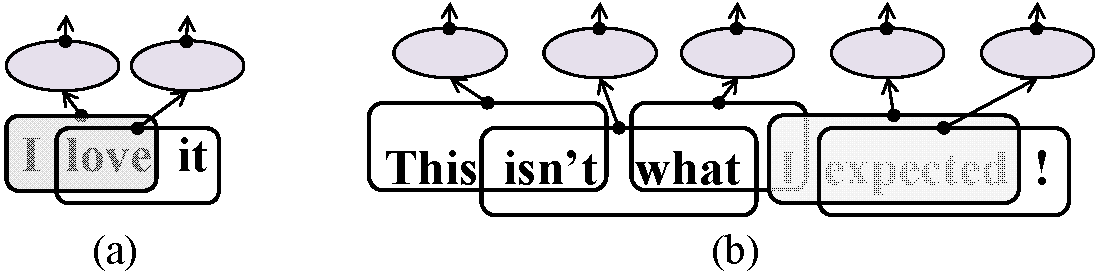
\includegraphics[width=3in]{txtconv}
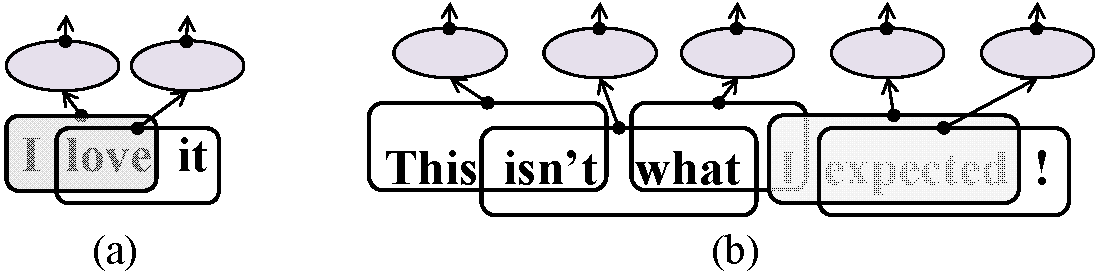
\includegraphics[width=2.6in]{txtconv}
\vspace{-0.15in}
\caption{\label{fig:txtconv} \footnotesize % \small
Convolution layer for variable-sized text.  
%%Computation units (ovals) share weights.  
%The number of units (ovals) depends on the document size.
%Region size 2 and stride 1. 
}
\end{figure}
%+++++++++++++++++++++++++++++++++++++++

%---
\subsection{\cnn\ vs. \bongrams}
\label{sec:cnn-vs-bow}
Traditional 
%text categorization 
methods represent each document {\em entirely} with 
one \bongram\ vector 
and then apply a classifier model such as SVM. 
However, 
since % the number of possible $n$-grams increases rapidly with $n$, 
high-order $n$-grams are 
susceptible to data sparsity, use of a large $n$ such as 20 is not only 
infeasible but also ineffective.  
%and to counteract it, it is necessary to include 
%not only high-order $n$-grams but also 
%lower-order $n$-grams in the vocabulary set; % (e.g., one has to concatenate the two vectors above); 
%otherwise, performance would be rather degraded.
%This implies that the discriminating power of 
%high-order $n$-grams, 
%%word sequences (as opposed to individual words in isolation), 
%which is obvious to humans, 
%cannot be fully exploited by the conventional methods based on \bongram\ vectors. 
%%%due to the data sparsity problem.  
Also 
note that a \bongram\ represents each $n$-gram by a one-hot vector 
and ignores the fact that some $n$-grams share constituent words.  
%
By contrast, \cnn\  % for text introduced above 
%is more robust in this regard.  
%This is because 
%instead of learning how to weight $n$-grams, 
internally learns {\em embedding of text regions} (given the consituent words as input) 
{\em useful for the intended task}.  
%{\em how to weight individual words in the sequence of a fixed size}, 
%in order to produce useful features for the intended task.  
Consequently, 
a large $n$ such as 20 can be used especially with the \bconv\ layer, 
which turned out to be useful on topic classification.
%as shown later. 
A neuron 
trained to assign a large value to, e.g., ``I love'' (and a small value to ``I hate'') 
is likely to assign a large value to ``we love'' (and a small value to ``we hate'') 
as well, {\em even though ``we love'' was never seen during training}.  
%Also, the effective region size of \cnn\ can be much larger than 
%the effective $n$ for the \bongram\ approach.  
We will confirm these points empirically later.  
%in Section \ref{sec:examples}. 

%---
\subsection{Extension: parallel \cnn}

%+++++++++++++++++++++++++++++++++++++++
\begin{figure}
\centering
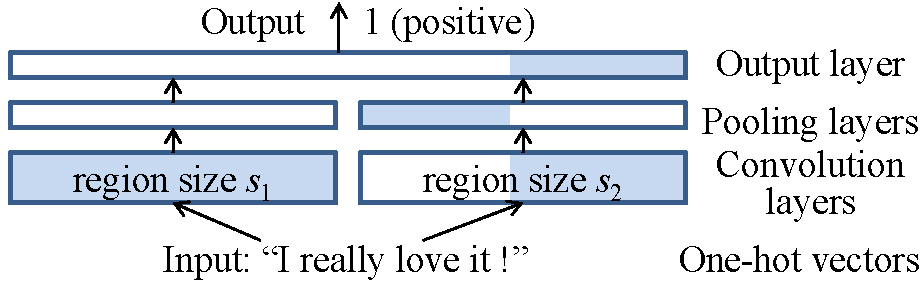
\includegraphics[width=3in]{multilaycnn}
%\vspace{-0.15in}
\caption{\label{fig:multilaycnn} \footnotesize % \small
CNN with two convolution layers in parallel.  
}
\end{figure}
%+++++++++++++++++++++++++++++++++++++++

We have described \cnn\ with the simplest network architecture that has one pair of 
convolution and pooling layers.  While this can be extended in several ways (e.g., 
with deeper layers), in our experiments, 
we explored {\em parallel \cnn}, which has 
two or more convolution layers in parallel\footnote{
  Similar architectures have been used for image.  
  \newcite{Kim14} used it for text, but it was on top of a word vector conversion layer. 
}, 
as illustrated in Figure \ref{fig:multilaycnn}. 
The idea is to learn multiple types of embedding of small text regions so that they can complement 
each other to improve model accuracy.  
In this architecture, 
multiple convolution-pooling pairs with different region sizes (and possibly 
different region vector representations) are given one-hot vectors as input and produce 
feature vectors for each region; the top layer takes the concatenation of the produced 
feature vectors as input.  

%-----
\section{Experiments}
\label{sec:experiment} 

We experimented with 
\cnn\ on two tasks, topic classification and sentiment classification. 
%in comparison with traditional methods that use \bongram\ vectors.  
%
Detailed information for reproducing the results 
is available on the internet along with our code.  

%-----
%\subsection{Experimental framework} 
\subsection{\cnn}
%\subsubsection{\cnn}
%\paragraph{\cnn}

%To experiment with \cnn, 
We fixed the activation function to 
rectifier {\small $\activ(x)=\max(x,0)$} and minimized square loss with $L_2$ 
regularization by 
{\em stochastic gradient descent} (SGD).  
%Our experiments focused on network architectures with 
%one pair of convolution and pooling layers.  
%However, note that it is possible to have more than one convolution-pooling layer 
%and/or to have fully-connected hidden layers above the convolution-pooling layer.  
%We tested several region sizes, pooling types, and the numbers of pooling units.  
%%while fixing the region stride to 1.  
%%and the padding size to $p-1$ where $p$ is the region size.  
We only used the 30K words that appeared most frequently in the training set; 
thus, for example, 
in \scnn\ with region size 3, a region vector is 90K dimensional.  
Out-of-vocabulary words were represented by a zero vector.  
On \bcnn, to speed up computation, 
we used {\em variable region stride} 
so that a larger stride was taken where repetition\footnote{
  For example, if we slide a window of size 3 over ``* * foo * *''
  where ``*'' is out of vocabulary, 
  a bag of ``foo'' will be repeated three times with stride fixed to 1.   
} 
of the same region vectors
can be avoided by doing so.  
Padding\footnote{
  As is commonly done, 
  to the beginning and the end of each document, special words that are treated as unknown words 
  (and converted to zero vectors instead of one-hot vectors) were added as `padding'.
  The purpose is to equally treat the words at the edge and words in the middle.  
}
size was fixed to $p-1$ where $p$ is the region size.  
%On \scnn, region stride was fixed to 1.  

We used two techniques commonly used with \cnn\ on image, which typically 
led to small performance improvements.  
One is {\em dropout} \cite{dropout12} optionally applied to the input to the top layer.  
The other is {\em response normalization} as in \cite{imagenetNips12}, 
which in our case scales the output of the pooling layer 
$\bz$ at each location by multiplying $(1 + |\bz|^2)^{-1/2}$.  

%-------------
\subsection{Baseline methods} 
%\subsubsection{Baseline methods} 
%\paragraph{Baseline methods} 
For comparison, we tested SVM
with the linear kernel and 
fully-connected neural networks
%\footnote{
%  While the description of a fully-connected neural network can be found 
%  in textbooks such as \cite{Bishop95}, it is worth mentioning that 
%  it can be considered as a special case of \cnn\ that 
%  regards the entire input data as $1 \times 1$ image.  
%}
(see e.g., \newcite{Bishop95})
with \bongram\ vectors as input.  
%We chose linear SVM as the state-of-the art predictor for this task.  
To experiment with fully-connected neural nets, 
as in \cnn, we minimized square loss 
with $L_2$ regularization 
and optional dropout
by SGD, and activation was fixed 
to rectifier.  
%---
To generate \bongram\ vectors, 
on topic classification, 
we first set each component to $\log(x+1)$ 
where $x$ is the word frequency in the document and then scaled them to unit vectors, 
which we found always % significantly 
improved performance over raw frequency.  
On sentiment classification, as is often done, we generated binary vectors and scaled them 
to unit vectors. 
%
We tested three types of \bongram: 
\bowone\ with $n \in \{1\}$, \bowtwo\ with $n \in \{1,2\}$, and \bowthree\ with $n \in \{1,2,3\}$; 
that is, \bowone\ is the traditional \bow\ vectors, and 
with \bowthree, each component of the vectors corresponds to either uni-gram, bi-gram, 
or tri-gram of words.  
%---
%To test the fully-connected neural networks, we tried several configurations in terms of 
%the number of hidden layers and the number of weight vectors in each layer and performed model 
%selection.  % (i.e., hyper-parameter selection).  
%%, and the chosen configuration was one hidden layer with 50 weight vectors.

%Note that the tested neural networks (either fully-connected or convolutional) 
%can be regarded as performing classification 
%with a linear model in the top/output layer while generating features (from the input features) 
%in the non-linear hidden layers.  
%In that sense, all the tested methods make predictions by a linear model, and the 
%difference between them is how they generate the features fed to the top layer. 
%The key differences are 
%whether/to what to degree word order is made use of, and whether non-linear embedding is 
%learned or not.  

We used SVMlight\footnote{
  \url{http://svmlight.joachims.org/}
}
for the SVM experiments.  
%\paragraph{\nbw} 
\tightpara{\nbw}
We also tested \nbw, which first appeared (but without performance report\footnote{
  WM12 instead reported the performance of an ensemble of NB and SVM as it performed better.  
}
) as NBSVM in WM12 \cite{WM12} and later with a small modification 
produced 
performance that exceeds state-of-the-art supervised methods 
on IMDB (which we experimented with) 
in MMRB14 \cite{MMRB14}.  
We experimented with the MMRB14 version, which 
generates binary \bongram\ vectors, multiplies the component 
for each $n$-gram $f_i$ with $\log(P(f_i|Y=1)/P(f_i|Y=-1))$
({\em NB-weight}) where the probabilities are estimated using the training data, 
and does logistic regression training.  
We used MMRB14's software\footnote{
  \url{https://github.com/mesnilgr/nbsvm}
} with a modification so that the regularization parameter
can be tuned on development data.  

%-----
\subsection{Model selection}
%\subsubsection{Model selection}
%\paragraph{Model selection}
\label{sec:protocol}
%Importantly, 
For all the methods, 
the hyper-parameters such as net configurations and 
regularization parameters were chosen 
based on the performance on the development data (held-out portion of the training data), 
and using the chosen hyper-parameters, the models were re-trained using all the training 
data.   
%The neural networks were trained by SGD with the following procedure: 
%first we perform 80 SGD iterations with learning rate $\eta$ and then 
%perform 20 SGD iterations with learning rate $0.1\eta$.  
%For all the methods, 
%%the training parameters (the initial learning rate $\eta$ and 
%%the $L_2$ regularization parameter for neural nets, 
%%and the regularization parameter for SVM) 
%%and network configuration parameters such as the number of weight vectors 
%hyper-parameters 
%were chosen by 
%either 5-fold cross validation on the training set or training/testing with the 4:1 split 
%of the training set.  When the training set is sufficiently large, we did the latter 
%to save time.  

%---
%\subsubsection{Implementation}
%%\paragraph{Implementation}
%We used SVM-light\footnote{
%  \url{http://svmlight.joachims.org/}
%} for the SVM experiments.  
%%For the neural networks, our implementation was built on {\em graphics processing unit (GPU)} 
%%for high-speed parallel processing, 
%%and it was designed to handle sparse high-dimensional vectors efficiently.  
%Our \cnn\ code on GPU 
%and detailed information for reproducing the results 
%will be available through the internet.  

%-----
\subsection{Data, tasks, and data preprocessing}
%We report the experimental results on three datasets: IMDB, \Elec, and RCV1. 
%\paragraph{IMDB: movie reviews}
\tightpara{IMDB: movie reviews}
The IMDB dataset 
%\footnote{
%  \url{http://ai.stanford.edu/~amaas/data/sentiment/}
%} 
\cite{MDPHNP11}
is a benchmark dataset for sentiment classification.  
%It consists of movie reviews from \url{www.imdb.com}.  
The task is to determine if the movie reviews are positive or negative.  
%Neutral reviews are not included in the data.  
%In this dataset, 
%the labels are balanced, i.e., there are the same number of positives and negatives 
%in both the training set and the test set, and the reviewed movies are 
%disjoint between the training set and test set so that detection of movie-specific features 
%(which would not generally be useful) should not lead to good results.  
Both the training and test sets consist of 25K reviews.  
For preprocessing, we tokenized the text so that emoticons such as ``:-)'' 
are treated as tokens and converted all the characters to lower case.  

%\paragraph{\Elec: electronics product reviews}
\tightpara{\Elec: electronics product reviews}
\Elec\ consists of electronic product reviews.  It is  
part of a large Amazon review dataset
%\footnote{
%  \url{https://snap.stanford.edu/data/web-Amazon.html}
%}
\cite{ML13}.  
%which consists of reviews of more than 
%20 types of products such as books and pet supplies.  
We chose electronics as it seemed to be very different from movies.    
Following the generation of IMDB \cite{MDPHNP11}, we chose the training set and 
the test set so that one half of each set consists of positive reviews 
and the other half is negative, regarding rating 1 and 2 as negative and 4 and 5 
as positive, and that the reviewed products are disjoint between the training set 
and test set.  Note that to extract text from the original data, 
we {\em only} used the {\em text section}, and we did {\em not} use the {\em summary section}.  
This way, we obtained a test set of 25K reviews (same as IMDB) 
and training sets of various sizes.  
The training and test sets are available on the internet\footnote{
  \url{riejohnson.com/cnn_data.html}
}. 
Data preprocessing was the same as IMDB.

%\paragraph{RCV1: topic categorization} 
\tightpara{RCV1: topic categorization} 
RCV1 
%\footnote{
%  \url{http://trec.nist.gov/data/reuters/reuters.html}
%} 
% is a benchmark dataset for topic classification.  
%It 
is a corpus of Reuters news articles % over a one-year period 
as described in LYRL04 \cite{rcv1}.  
%We used the ``RCV1-v2'' labeling, namely, the class labels corrected by LYRL04 
%for consistency of label hierarchy.  
%Note that although LYRL04 provides feature vectors obtained by applying 
%lower-case conversion, stopword removal, portal stemming, and tfidf feature weighting, 
%we could not use them since our methods require word order information that was lost 
%in their processing.  
%-- 
RCV1 has 103 topic categories 
in a hierarchy, 
%in a tree structure, 
and one document may 
be associated with more than one topic.  
%have more than one topic associated with it.  
Performance on this task (multi-label categorization) 
is known to be sensitive to thresholding strategies, 
which are algorithms additional to the models we would like to test.  
Therefore, we also experimented with single-label categorization 
to assign one of 55 second-level topics to each document 
% (excluding the documents that have more than one labels), 
to directly evaluate models.  
%Following the previous studies \cite{}, we removed documents with multiple second-level topics.  
For this task, 
we used the documents from a one-month period % (July'97) 
as the test set and generated various sizes of 
training sets from the documents with {\em earlier} dates.  
%with dates {\em earlier} than the test documents. 
%% following LYRL04. 
%--
%The training data and test data of the RCV1 experiments are summarized in Table \ref{tab:rcv-data}.   
Data sizes are shown in Table \ref{tab:rcv-data}.  
%Following 
As in 
LYRL04, we used the concatenation of the headline and text elements. 
Data preprocessing was the same as IMDB except that we used the stopword list 
provided by LYRL04 and regarded numbers as stopwords.  
%Unlike LYRL04, we did not apply stemming or tfidf 
%weighting.

%+++++++++++++++
\begin{table}
\begin{center}
\begin{footnotesize}
\begin{tabular}{|c|c|r|r|r|} 
\hline
   & label          &\multicolumn{1}{|c|}{\#train}&\multicolumn{1}{|c|}{\#test}& \#class \\
\hline
Table \ref{tab:all}  & single  & 15,564 & 49,838 & 55 \\% (2nd-level) \\
\hline
Fig. \ref{fig:size}  & single  & varies &  %% Aug'96--Oct'96 
                                          49,838 & 55 \\% (2nd-level) \\ 
\hline                                                                
Table \ref{tab:rcv-multi}   & multi   & 23,149 & 781,265 & 103 \\
\hline
\end{tabular}
\end{footnotesize}
\vspace{-0.1in}
\caption{ \label{tab:rcv-data} \small 
RCV1 data summary.  
%The exact training/test split 
%will be available through the internet.  %cmt: can't say "will be"; too many mentions of internet. 
}
\end{center}
\end{table}
%+++++++++++++++ 

%----- 
\subsection{Performance results}
Table \ref{tab:all} shows the error rates of \cnn\ in comparison with 
the baseline methods. % on all three datasets.  
The first thing to note is that on all the datasets, 
the best-performing \cnn\ outperforms the baseline methods, 
which demonstrates the effectiveness of our approach.  
  
To look into the details, 
let us first focus on \cnn\ with one convolution layer 
(\scnnpfx- and \bcnn\ in the table).  
On sentiment classification (IMDB and \Elec), 
the configuration chosen by model selection % (using the development set) 
was: region size 3, stride 1, 1000 weight vectors, and max-pooling 
with one pooling unit, for both types of \cnn; 
\scnn\ outperforms \bcnn, as well as all the baseline methods except for one.  
%Region size 4 and 5 also produced similar results.  
Note that with a small region size and max-pooling, 
if a review contains a short phrase that conveys strong sentiment 
(e.g., ``A great movie!''), the review could receive a high score irrespective of the rest of the review. 
It is sensible that this type of configuration is effective on sentiment classification.  

By contrast, on topic categorization (RCV1), 
the configuration chosen for \bcnn\ by model selection was: region size 20, variable-stride$\ge$2, 
average-pooling with 10 pooling units, and 1000 weight vectors, 
which is very different from sentiment classification.  
This is presumably because 
on topic classification, a larger context would be more predictive 
than short fragments ($\rightarrow$ larger region size), 
the entire document matters ($\rightarrow$ the effectiveness of average-pooling), 
and the location of predictive text also matters ($\rightarrow$ multiple pooling units). 
The last point may be because news documents tend to have crucial sentences 
(as well as the headline) at the beginning.  
On this task, while both \scnnpfx\ and \bcnn\ outperform the baseline methods, \bcnn\ outperforms \scnn,  
which indicates that in this setting 
the merit of having fewer parameters is larger than the benefit of keeping word order 
in each region.  
 
Now we turn to parallel \cnn. %, as illustrated in Figure \ref{fig:multilaycnn}.   
On IMDB, \sscnn, which has two seq-convolution layers 
(region size 2 and 3; 1000 neurons each; followed by one unit of max-pooling each), 
outperforms \scnn.  With more neurons (3000 neurons each; Table \ref{tab:imdb-prev}) it 
further exceeds 
the best-performing baseline, which is also the best previous supervised result.    
%On \Elec, \sscnn\ (region size 3 and 4; 1000 neurons each) 
%slightly outperforms \scnn.  
%Both used one unit of max-pooling as in \scnn.  
We presume the effectiveness of \sscnn\ indicates that the length of predictive text regions 
is variable.  

The best performance 7.67 on IMDB was obtained by `\ssbcnn', 
equipped with three layers in parallel: 
two seq-convolution layers (1000 neurons each) as in \sscnn\ above and  
one layer (20 neurons) that {\em regards the entire document as one region} and 
represents the region (document) by a \bongram\ vector (\bowthree)
as input to the computation unit; 
in particular, we generated \bowthree\ vectors by multiplying the NB-weights with binary vectors, 
motivated by the good performance of \nbw.  
This third layer is a \bow-convolution layer\footnote{
  It can also be regarded as a fully-connected layer that takes \bowthree\ vectors as input. 
}
with one region of variable size that takes 
one-hot vectors with $n$-gram vocabulary as input to learn document embedding.  
The \ssbcnn\ for \Elec\ in the table is the same except that the regions sizes of seq-convolution layers are 
3 and 4.  On both datasets, performance is improved over \sscnn.
The results % demonstrate extendability of \cnn\ and 
suggest that what can be learned through these three layers are distinct enough 
to complement each other.  
The effectiveness of the third layer indicates that not only short word sequences 
but also global context in a large window may be useful on this task; thus, inclusion of a 
\bconv\ layer with $n$-gram vocabulary with a large fixed region size might be even more effective, 
providing more focused context, 
but we did not pursue it in this work.  

%%(i.e., replacing \bowone\ with \bowtwo), 
%but further adding tri-grams 
%%(i.e., replacing \bowtwo\ with \bowthree) 
%did not improve performance much. 

\tightpara{Baseline methods} 
Comparing the baseline methods with each other, on sentiment classification, 
reducing the vocabulary to the most frequent $n$-grams notably hurt 
performance (also observed on \nbw\ and NN)
even though some reduction is a common practice. 
Error rates were clearly improved by addition of bi- and tri-grams. 
%Further adding tri-grams improved performance but not much when 
%vocabulary is reduced to size 30K, presumably because addition of tri-grams 
%pushed out useful uni- and bi-grams.  
By contrast, on topic categorization, % addition of 
bi-grams only slightly improved accuracy, and reduction of vocabulary did not 
hurt performance.  
\nbw\ is very strong on IMDB and poor on RCV1; its effectiveness appears to be 
data-dependent, 
%which is consistent with WM12's observation.  
as also observed by WM12. 
%We also tested fully-connected neural networks with the features of \nbw, but it performed no better 
%than \nbw.  


%+++++++++++++++
\begin{table}
\begin{center}
\begin{small}
\begin{tabular}{|l|r|r|r|} 
\hline
%rcv1: use stopwords for all 
methods        & IMDB  & Elec  &  RCV1 \\  % 
\hline
%--                                 % st       % rcv1:ns
%SVM \bowone\ (30K)  & 11.45 & 11.70 & 10.83 \\ % 
%SVM \bowtwo\ (30K)  & 10.18 &  9.33 & 10.62 \\ % 
SVM \bowthree\ (30K)& 10.14 &  9.16 & 10.68 \\ % 
\hline
SVM \bowone\ (all)  &    11.36 &    11.71 &     10.76 \\ 
SVM \bowtwo\ (all)  &     9.74 &     9.05 &     10.59 \\ 
SVM \bowthree\ (all)&     9.42 &     8.71 &     10.69 \\
\hline
NN \bowthree\ (all) &     9.17 &     8.48 &     10.67 \\ % 
                                               % imdb:nosort,1e-5,0.025,do,50nodes
                                               % elec:nosort,1e-4,0.1,do,50nodes
                                               % rcv1:nosort,1e-5,0.5,500nodes
\hline
%\nbw\ \bowone\ (all)  &    11.39  &   11.56 &       .   \\ % 11.20,11.27 % 
%\nbw\ \bowtwo\ (all)  &     8.44  &    8.38 &       .   \\ % 11.63,11.53 % 
\nbw\ \bowthree\ (all)&     8.13 &     8.11 &     13.97 \\ % 11.92,12.24 % 
\hline \hline
\bcnn\      &     8.66 &     8.39 &{\bf 9.33}\\ 
\scnn\      &     8.39 &     7.64 &     9.96 \\ 
\hline
\sscnn\     &     8.04 &     7.48 &\multicolumn{1}{|c|}{--}\\
\ssbcnn\    &{\bf 7.67}&{\bf 7.14}&\multicolumn{1}{|c|}{--}\\
\hline
\end{tabular}
\end{small}
\vspace{-0.1in}
\caption{ \label{tab:all} \small
Error rate (\%) 
comparison with bag-of-$n$-gram-based methods.
Sentiment classification on IMDB and \Elec\
(25K training documents) 
and 55-way topic categorization on RCV1 (16K training documents).  
%See Table \ref{tab:rcv-data} for training/test data. 
`(30K)' indicates that the 30K most frequent $n$-grams were used, 
and `(all)' indicates that all the $n$-grams (up to 5M) were used.  
\cnn\ used the 30K most frequent words.  
}
\end{center}
\end{table}
%+++++++++++++++

%+++++++++++++++
\begin{table}
\begin{center}
\begin{small}
\begin{tabular}{|l|r|c|} 
%\hline
%methods       & Error rate & resource\\
\hline
%linear model [MDPHNP11] & 11.77 & -- \\
SVM \bowtwo\ [WM12]    & 10.84 & -- \\
WRRBM+\bow\ [DAL12]    & 10.77 & -- \\
NB+SVM \bowtwo\ [WM12] & 8.78  & ensemble\\
\nbw\ \bowthree\ [MMRB14]& 8.13  & -- \\
\hline
%Word vectors [MDPHNP11]& 11.11 & unlabeled data\\ 
Paragraph vectors [LM14] & 7.46 & unlabeled data\\
%Sentence vectors+\nbw &\multirow{2}{*}{7.43}& ensemble \& \\
%\multicolumn{1}{|r|}{+LM-RNN [MMRB14]}&     & unlabeled data \\
\hline  
\sscnn\ (3K$\times$2) [Ours]  &     7.94  & -- \\   
\ssbcnn\ [Ours] &{\bf 7.67} & -- \\
\hline
\end{tabular}
\end{small}
\end{center}
%\caption{ \label{tab:rcv-multi} Caption}
\vspace{-0.2in}
\caption{ \label{tab:imdb-prev} \small
Error rate (\%) comparison with previous best methods 
%(single-classifier supervised methods only) 
on IMDB. 
%The table shows single-classifier supervised learning results only.  
%$r$ and $s$ for \bcnn\ and \scnn\ are the region size and stride, respectively. \\
}
\end{table}
%+++++++++++++++

%\subsubsection{Comparison with state-of-the-art results}
%\paragraph{Comparison with state-of-the-art results} 
\tightpara{Comparison with state-of-the-art results} 
%\paragraph{IMDB}
%In Table \ref{tab:imdb-prev} we show the previous results on IMDB.  
%We also note that 
%our linear model results are better than the similar settings of the previous studies 
%such as \cite{MDPHNP11}'s linear model with their version of \bowone, 
%and \cite{WM12}'s linear SVM with their version of \bowtwo.  
%This is presumably because we used a sufficient number of words (30K) 
%whereas \cite{MDPHNP11} used only 2000 words, and 
%because \cite{WM12} limited their bi-grams to be alphabet only, which we found hurt accuracy, 
%and we did not limit our $n$-grams.  
As shown in Table \ref{tab:imdb-prev}, 
the previous best supervised result on IMDB is 8.13 by \nbw\ with \bowthree\ (MMRB14), 
and our best error rate 7.67 is better by nearly 0.5\%.  
%
\cite{LM14} reports 7.46 with the semi-supervised method that learns low-dimensional 
vector representations of documents from unlabeled data.  
%and MMRB14 reports 7.43 with the ensemble of three independently-trained models including 
%a semi-supervised model.  
Their result is not directly comparable with our supervised results due to use of additional resource.  
Nevertheless, our best result rivals their result.  

%{\em paragraph vectors}.  
%However, 
%their experiments with IMDB used unlabeled data as additional resource (which we did 
%not use), and we cannot simply compare it with the supervised learning results 
%without additional resources.    
%---
%However, a potential disadvantage 
%of \cite{LM14}'s method is that it requires iterative optimization for learning paragraph 
%vectors not only at the time of training but also at the time of making predictions, 
%which would slow down predictions.  Our method does not have this issue.  

%---
%\paragraph{RCV1}
We tested \bcnn\ on the multi-label topic categorization task on RCV1
%on the {\em LYRL2004} split as defined in LYRL04 
to compare with LYRL04.  
%The task is to assign one or more topic classes to each document, choosing from 103 classes. 
%and it can be regarded as performing 103 binary classification tasks.  
%With the LYRL2004 split, the training set consists of 23,149 documents with the earliest 
%dates (Aug'96), and the test set consists of the rest, 781,265 documents (Sept'96--Aug'97).  
%The evaluation metrics are micro-averaged and 
%and macro-averaged $F_1$. 
%%$F_{1.0} = 2pr/(p+r)$ where $p$ and $r$ are precision and recall, respectively.  
%
%On this task, % in general, given the predictor output $f(\bx)$ for each class, 
%whether to assign a label needs to be determined by thresholding predictor output 
%for each class.  
%, and performance depends on not only the model quality but also the thresholding 
%strategy, as noted by LYRL04.  
We used the same thresholding strategy as LYRL04. 
%, so that comparison can focus on the model quality.  
%The network configuration chosen for \bcnn\ was the same as in the single-label experiments.   
As shown in Table \ref{tab:rcv-multi}, 
\bcnn\ outperforms LYRL04's best results % obtained by linear SVM, 
even though our data preprocessing is much simpler (no stemming and no tf-idf weighting).  
%Note that as mentioned above, we could not use the preprocessed data provided by LYRL04, 
%and our pre-processing is simpler (no stemming and no tf-idf weighing).  For this reason, we also
%show the linear model results with \bow\ using our preprocessing in the table.  
%\bcnn\ outperforms this linear model as well.  


%+++++++++++++++
\begin{table}
\begin{center}
\begin{small}
\begin{tabular}{|c|c|c|} 
\hline
models                         & micro-F & macro-F \\
\hline
LYRL04's best SVM   & 81.6   & 60.7    \\
\hline
%Linear (square loss) \bowone\  & 81.7  & 62.3  \\
\bcnn\                          &{\bf 84.0}&{\bf 64.8}\\ % 1k
%\bcnn\ & 84.1  & 65.8  \\ % 1k w/ different a thresholding strategy.  
\hline
\end{tabular}
\end{small}
\vspace{-0.1in}
\caption{ \label{tab:rcv-multi} \small
RCV1 micro-averaged % F measure 
and macro-averaged F-measure results 
on multi-label task with LYRL04 split.   
%See Table \ref{tab:rcv-data} for training/test data.
}
\end{center}
\end{table}
%+++++++++++++++

%--------------
%\subsubsection{Comparison with previous \cnn} %\ for sentence classification} 
%\paragraph{Previous \cnn}
\tightpara{Previous \cnn}
We focus on the sentence classification studies due to its relation to text categorization.  
\newcite{Kim14} studied fine-tuning of pre-trained word vectors to produce input to 
%one-layer \cnn\ with one-unit max-pooling.  
parallel \cnn.  
He reported that performance was poor 
when word vectors were trained as part of \cnn\ training (i.e., no additional method/corpus).  
On our tasks, 
we were also unable to outperform the baselines with this type of model. 
%%this type of model also underperformed the baselines. 
%%(using our code as his code did not scale to our tasks). 
%
%rmv?
Also, with our approach, a system is simpler with one fewer layer 
-- no need to tune the dimensionality of word vectors or meta-parameters for word vector learning.  
%As mentioned earlier, 
%the word vector learning layer in this setting can be viewed as a special case of 
%convolution layer with region size {\em one}, and 
%region size one is apparently not suitable for these tasks 
%in supervised settings.  

\newcite{KGB14} proposed complex modifications of \cnn\ 
for sentence modeling.  Notably, given word vectors $\in \mathbb{R}^d$, 
their convolution with \numNeuron\ feature maps produces for each region a matrix $\in \mathbb{R}^{d \times \numNeurono}$ 
(instead of a vector $\in \mathbb{R}^\numNeurono$ as in standard \cnn). 
%which makes a model complex.  
%though 
%the effect of this modification alone is not clear.  
Using the provided code, we found that their model is too resource-demanding 
for our tasks.  
On IMDB and \Elec\footnote{
  We could not train adequate models on RCV1 on either Tesla K20 or M2070 
  due to memory shortage. 
}
the best error rates we obtained
by training with various configurations that fit in memory 
for 24 hours each on GPU (cf. Fig \ref{fig:time}) 
were 10.13 and 9.37, respectively, %which are only as good as SVM \bowtwo\ with reduced vocabulary.  
which is no better than SVM \bowtwo.  
Since excellent performances were reported on short sentence classification, 
we presume that their model is optimized for short sentences, but not for text categorization in general.   
% KGB14: 10.13 (IMDB, dim75, k4, p7, n10), 9.37 (\Elec)

%Thus, on text categorization, the \cnn\ models we propose have an advantage of 
%higher accuracy and simplicity.  
%%and faster training.  

%%+++++++++++++++++++++++++++++++++++++++
%\begin{figure*}
%\centering
%%\includegraphics[width=5.8in]{graphs}
%\includegraphics[width=5in]{graphs}
%\vspace{-0.15in}
%\caption{\label{fig:graphs} \small
%Performance dependency on: (a) and (b) training data size and (c) the number of neurons. 
%%(a) and (b): 
%%In relation to training data size; 
%%(c) in relation to the number of weight vectors.  
%%\bowtwo\ (RCV1) and \bowthree\ (\Elec\ and RCV1) are not shown 
%%because they almost overlap with the existing lines.  
%%For readability, the baseline methods that almost overlap with the existing lines 
%%are not shown.  
%}
%\end{figure*}
%%+++++++++++++++++++++++++++++++++++++++

%+++++++++++++++++++++++++++++++++++++++
\begin{figure}[t]
\centering
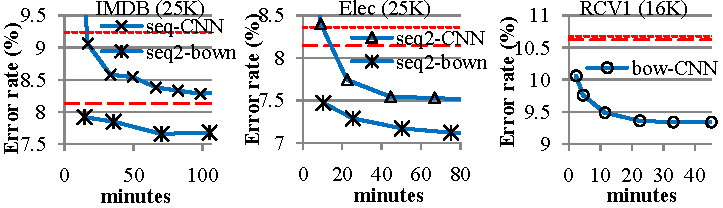
\includegraphics[width=3.2in]{time2}
\vspace{-0.3in}
\caption{\label{fig:time} \small % \footnotesize % \small
Training time (minutes) on 
Tesla K20. 
The horizontal lines are % the error rates of 
the best-performing baselines.  
}
\end{figure}
%+++++++++++++++++++++++++++++++++++++++
%+++++++++++++++++++++++++++++++++++++++
\begin{figure}[t]
\centering
%\includegraphics[width=5.8in]{graphs}
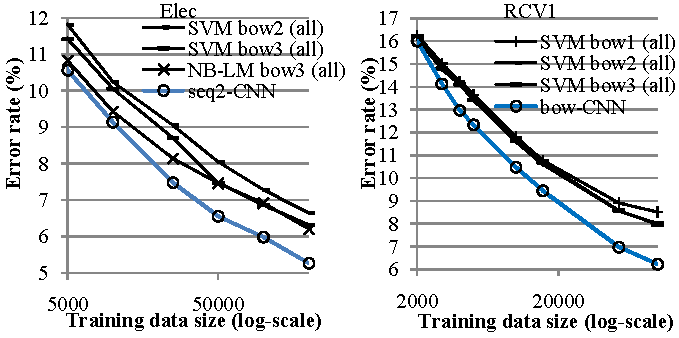
\includegraphics[width=3.2in]{size}
\vspace{-0.3in}
\caption{\label{fig:size} \small
Error rate in relation to training data size. 
For readability, only representative methods are shown. 
}
\end{figure}
%+++++++++++++++++++++++++++++++++++++++
%-----
%\subsection{Performance dependency on various factors} 
% training data size and the number of parameters} 
%\subsection{Empirical analysis} 
%\subsection{Performance dependency analysis}
\tightpara{Performance dependency}
%Figure \ref{fig:graphs} (c) plots
%performance dependency on the number of 
%weight vectors (or neurons) in the convolution layer on RCV1.  
%The results indicate that it is important to have sufficient number of 
%weight vectors.  
%Since the task is 55-way classification, having fewer neurons than 55 degrades 
%performance.  
%%cmt say something. 
%
\cnn\ training is known to be expensive, compared with, e.g., linear models -- 
linear SVM with \bowthree\ on IMDB only 
takes 9 minutes using SVMlight (single-core) on a high-end Intel CPU.  
Nevertheless, with our code on GPU, \cnn\ training only takes minutes (to a few hours)
on these datasets shown in Figure \ref{fig:time}.  

Finally, the results with training sets of various sizes on \Elec\ and RCV1 
are shown in Figure \ref{fig:size}.

%Error rates become better than the best-performing baseline within 
%3--15 minutes and reach nearly the best in 20--50 minutes. % depending on these datasets.  
%cmt say more?

%-----
\subsection{Why is \cnn\ effective?} 
\label{sec:examples}
In this section we explain the effectiveness of \cnn\ through 
looking into what it learns from training.  

First, for comparison,
we show the $n$-grams that SVM with \bowthree\ found to be the most predictive; i.e., 
%more precisely, 
the following $n$-grams were assigned the 10 largest weights by SVM with binary features on \Elec\ 
%(\#train=25K),  % saving space ...
for the negative and positive class, respectively: 
\vspace{-0.1in}
%\begin{small}
\begin{itemize} \itemsep1pt \parskip0pt \parsep0pt
\item 
{\small
  poor, useless, returned, not worth, return, worse, disappointed, terrible, worst, horrible  % n1n2n3nsallb1u1
%  useless, poor, returned, worse, return, not worth, disappointing, horrible, terrible, disappointed % 30k
}
\item
{\small
  great, excellent, perfect, love, easy, amazing, awesome, no problems, perfectly, beat
%  excellent, great, amazing, perfect, awesome, love, no problems, easy, perfectly, my only
}  
\end{itemize}
\vspace{-0.05in}
%\end{small}  
Note that, even though SVM was also given bi- and tri-grams, 
the top 10 features chosen by SVM with binary features are mostly uni-grams; 
furthermore, the top 100 features (50 for each class) include 28 bi-grams but only four tri-grams. 
This means that, with the given size of training data, SVM still heavily counts on 
uni-grams, which could be ambiguous, and cannot fully take advantage of higher-order 
$n$-grams.
%---  nbw svm
% never worked, not a good, never received, not received, worse, stay away, very disappointed, useless, not worth, is the worst
% highly recommend this, . highly recommended, i recommend this, this is it, 'm very pleased, can't go wrong, a must have, awesome, love this, great product
%---  nbw lr
% never worked, not a good, very disappointed, useless, is the worst, never received, not received, not buy, 2 stars, stay away
% highly recommend this, i recommend this, . highly recommended, this is it, excellent, . no problems, a must have, great, perfect !, definitely worth
By contrast, 
NB-weights tend to promote $n$-grams with a larger $n$; the 100 features that were assigned 
the largest NB-weights are 7 uni-, 33 bi-, and 60 tri-grams.  
%the top 100 features of \nbw\ 
%(measured by the NB-weight times the linear-model weight) include 
%%21 uni-, 39 bi-, and 40 tri-grams.  % svm
%28 uni-, 44 bi-, and 28 tri-grams.  % logistic regression
%The difference is due to the fact that the NB-weights tend to be 
%larger on $n$-grams with a larger $n$.  
However, as seen above, NB-weights do not always lead to the best performance.  

In Table \ref{tab:bv}, 
we show some of text regions learned by \scnn\ to be predictive on \Elec.  
%The net configuration is % the one from Table \ref{tab:all}, which has 
%1000 neurons (weight vectors) in the convolution layer.  
This net has one convolution layer with region size 3 and 1000 neurons; 
thus, embedding by the convolution layer produces a 1000-dim vector 
for each region, which (after pooling) serves as features in the top layer
where weights are assigned to the 1000 vector components.  
%Recall that 
%the output/activation of the 1000 neurons (the results of embedding) serve as features 
%(after pooling) in the top layer, 
%and the top layer assigns weights to the features.  
In the table, N$i$/P$i$ indicates the component that received 
the $i$-th highest weight in the top layer 
%(thus $i$-th most predictive) 
for the negative/positive class, respectively. The table shows the text regions 
(in the training set) whose embedded vectors have a large value
in the corresponding component, i.e., predictive text regions.  

Note that the embedded vectors for the text regions listed in the same row 
are close to each other as they have a large value in the same component. 
That is, Table \ref{tab:bv} also shows that
the {\em proximity of the embedded vectors} tends to reflect the {\em proximity  
in terms of the relations to the target classes} (positive/negative sentiment). 
This is the effect of embedding, which helps classification by the top layer.  

%Note that, e.g., ``is so bad'' cannot be shorter for detection of 
%the negative sentiment since ``so bad'' could be a part of ``not so bad''; thus, 
%tri-gram is indeed helpful for accurate prediction.  

%+++++++++++++++
\begin{table}
\begin{center}
\begin{footnotesize}
\begin{tabular}{|c|p{2.5in}|} 
\hline
{\small N1} & {\small completely useless ., return policy .} \\
{\small N2} & {\small it won't even, but doesn't work} \\
{\small N3} & {\small product is defective, very disappointing !} \\
{\small N4} & {\small is totally unacceptable, is so bad} \\
{\small N5} & {\small was very poor, it has failed} \\
%{\small N6} &{\small it isn't worth, no longer work} \\
\hline
{\small P1} & {\small works perfectly !, love this product} \\
{\small P2} & {\small very pleased !, super easy to, i am pleased} \\
{\small P3} & {\small 'm so happy, it works perfect, is awesome !} \\
{\small P4} & {\small highly recommend it, highly recommended !} \\  % would highly recommend
{\small P5} & {\small am extremely satisfied, is super fast} \\
%{\small P6} & {\small solid construction ., quality is wonderful} \\
\hline
\end{tabular}
\end{footnotesize}
\vspace{-0.1in}
\caption{ \label{tab:bv} \small
Examples of predictive text regions in the training set. 
%training 
%text regions that highly activate \scnn's convolution-layer neurons on \Elec.  
%\scnn\ with region size 3, stride 1, and 1000 neurons.  
%N$i$/P$i$ indicates the $i$-th most influential neuron 
%in detecting the negative/positive class, respectively. 
}
\end{center}
\end{table}
%+++++++++++++++

%As is mentioned in Section \ref{sec:cnn-vs-bow}, 
%the methods that rely on bag of high-order $n$-grams can
%suffer from data sparsity.  This is because with conventional methods, 
With the \bongram\ representation, 
only the $n$-grams that 
appear in the training data can participate in prediction. 
%but 
%the vocabulary overlap between training data and test data rapidly 
%decreases as $n$ increases.  
%\footnote{
%  For example,  
%  the 25K \Elec\ training documents contain 1.6 million types of tri-grams 
%  and so do the 25K test documents, but only 391K tri-grams appear in both. 
%}.  
By contrast, 
one strength of \cnn\ is that $n$-grams (or text regions of size $n$) 
{\em can contribute to accurate prediction even if they did not appear in the training data}, 
as long as (some of) their constituent words did, 
%This is because vector representation of each text region is 
%based on their constituent words. % (see Section \ref{sec:scnn}).  
because input of embedding is the constituent words of the region.   
%
%+++++++++++++++
\begin{table}
\begin{center}
\begin{footnotesize}
\begin{tabular}{|p{2.9in}|} 
\hline
{\small 
%printer printed garbage,  % router became defective, 
%cursor won't move,  % m240 can't display, 
%%was kindof disappointing, makes spectacularly bad, 
were unacceptably bad, is abysmally bad,  % , gets increasingly bad, 
were universally poor, %% were dissappointingly poor, . laughable poor, 
%%was moderatley disappointed, 
was hugely disappointed, was enormously disappointed, 
%no playlists supported, 
is monumentally frustrating,  are endlessly frustrating
%is awkwardly uncomfortable, 
%%horrible crunching static, 
%no troubleshooting help
%%lasted 101 minutes 
}\\
\hline
{\small 
best concept ever, best ideas ever, best hub ever, %% best manufacturer ever, 
am wholly satisfied, 
am entirely satisfied, am incredicbly satisfied, 
%am completly satisfied, 
%%*am real pleased, *'m extrememly happy, 
'm overall impressed, am awfully pleased, 
am exceptionally pleased, 'm entirely happy, 
%%*am exteremly happy
%produces fantastic quality, showed amazing performance, 
are acoustically good, is blindingly fast, 
%gives unbelievably clear, 
%offers outstanding portability
%%*would deffinetly buy, *would definantly buy, *would definetley buy, *would absolutly buy, *``would definatley buy
}\\
\hline
\end{tabular}
\end{footnotesize}
\vspace{-0.1in}
\caption{ \label{tab:bv-tstonly} \small
Examples of text regions that contribute to prediction. 
%that highly activate \scnn's neurons trained on \Elec.  
They are from the {\em test set}, and they 
did {\em not} appear in the training set, either entirely or partially as bi-grams.  
}
\end{center}
\end{table}
%+++++++++++++++
%
To see this point, in Table \ref{tab:bv-tstonly} we show the text regions from the {\em test set}, 
which {\em did not appear in the training data}, either entirely or partially as bi-grams, 
and yet whose embedded features have large values in the heavily-weighted (predictive) component 
thus contributing to the prediction.  
There are many more of these, and we only show a small part of them that fit certain patterns.  
One noticeable pattern is (be-verb, adverb, sentiment adjective) such as 
``am entirely satisfied'' and ``'m overall impressed''.  
These adjectives alone could be ambiguous as they may be negated.  To know that the 
writer is indeed ``satisfied'', we need to see the sequence ``am satisfied'', 
but the insertion of adverb such as ``entirely''  
is very common.  ``best X ever' is another pattern that a discriminating pair of words are not adjacent to 
each other.  These patterns require tri-grams for disambiguation, and 
\scnn\ successfully makes use of them even though the exact tri-grams were not seen during training, 
as a result of learning, e.g., ``am X satisfied'' with non-negative X 
(e.g., ``am very satisfied'', ``am so satisfied'') 
to be predictive of the positive class through training. 
%
%In other words, \cnn\ retains information that 
%``am very satisfied'' consists of three words ``am'', ``very'', and ``satisfied'' in this order, 
%but bag-of-$n$-gram approaches lose it by treating $n$-grams as atoms.  
%Due to this extra information, 
That is, 
\cnn\ can effectively use word order when \bongram-based approaches fail.  

%-----
\section{Conclusion}
\label{sec:conclude}
This paper showed that \cnn\ provides an alternative mechanism for effective use of word order 
for text categorization through direct embedding of small text regions, 
different from the traditional \bongram\ approach or word-vector \cnn.  
With the parallel \cnn\ framework, several types of embedding 
can be learned and combined so that they can complement each other 
for higher accuracy.  
State-of-the-art performances on sentiment classification and topic classification were 
achieved using this approach. 

\section*{Acknowledgements}
We thank the anonymous reviewers for useful suggestions.  
The second author was supported by NSF IIS-1250985 and NSF IIS-1407939.  

%\subsubsection*{References}
\bibliographystyle{naaclhlt2015}
\bibliography{cnn-text-naacl-arxiv}

\end{document}

% LocalWords:  multi embeddings UA eq Xone Xtwo SGD IMDB RCV MNISTvar datasets
% LocalWords:  unregularized GPU BoW RGB dimensionality unaffordably cccccccc
% LocalWords:  cnn
